\chapter{Gradient methods}


\section{Minimum of a function}

Let $f: \mathbb{R}^N \rightarrow \mathbb{R}$ be continuous and differentiable in $\mathbb{R}^N$.
\begin{descriptionlist}
    \item[Stationary point] \marginnote{Stationary point}
        $\vec{x}^*$ is a stationary point of $f$ iff: 
        \[ \nabla f(\vec{x}^*) = \nullvec \]

    \item[Local minimum] \marginnote{Local minimum}
        $\vec{x}^* \in \mathbb{R}^N$ is a local minimum of $f$ iff:
        \[ \exists \varepsilon \in \mathbb{R} \text{ s.t. } 
            f(\vec{x}^*) \leq f(\vec{x}) \text{ } \forall \vec{x} \in \mathbb{R}^N: \Vert \vec{x} - \vec{x}^* \Vert < \varepsilon \]
        
    \item[Strict local minimum] \marginnote{Strict local minimum}
        $\vec{x}^* \in \mathbb{R}^N$ is a strict local minimum of $f$ iff:
        \[ \exists \varepsilon \in \mathbb{R} \text{ s.t. }
            f(\vec{x}^*) < f(\vec{x}) \text{ } \forall \vec{x} \in \mathbb{R}^N: \Vert \vec{x} - \vec{x}^* \Vert < \varepsilon \]

    \item[Global minimum] \marginnote{Global minimum}
        $\vec{x}^* \in \mathbb{R}^N$ is a global minimum of $f$ iff:
        \[ f(\vec{x}^*) \leq f(\vec{x}) \text{ } \forall \vec{x} \in \mathbb{R}^N \]
        
    \item[Strict global minimum] \marginnote{Strict global minimum}
        $\vec{x}^* \in \mathbb{R}^N$ is a strict global minimum of $f$ iff:
        \[ f(\vec{x}^*) < f(\vec{x}) \text{ } \forall \vec{x} \in \mathbb{R}^N \]
\end{descriptionlist}

Note that $\max \{ f(x) \} = \min \{ -f(x)$ \}. 


\subsection{Optimality conditions}

\begin{description}
    \item[First-order condition] \marginnote{First-order condition}
        Let $f: \mathbb{R}^N \rightarrow \mathbb{R}$ be continuous and differentiable in $\mathbb{R}^N$.
        \[ \text{If } \vec{x}^* \text{ local minimum of } f \Rightarrow \nabla f(\vec{x}^*) = \nullvec \]

    \item[Second-order condition] \marginnote{Second-order condition}
        Let $f: \mathbb{R}^N \rightarrow \mathbb{R}$ be continuous and twice differentiable.
        \[ 
            \text{If } \nabla f(\vec{x}^*) = \nullvec \text{ and } \nabla^2 f(\vec{x}^*) \text{ positive definite} \Rightarrow 
            \vec{x}^* \text{ strict local minimum of } f 
        \]
\end{description}

As the second-order condition requires computing the Hessian matrix, which is expensive, in practice only the first-order condition is checked.



\section{Descent methods}

\marginnote{Descent methods}
Descent methods are iterative methods that have the property:
\[ f(\vec{x}_k) < f(\vec{x}_{k-1}) \]

The iteration is defined as:
\[ \vec{x}_k = \vec{x}_{k-1} + \alpha_{k-1}\vec{p}_{k-1} \]
where $\vec{p}_{k-1} \in \mathbb{R}^N$ is the search direction and \marginnote{Search direction\\Step length}
$\alpha_{k-1} \in \mathbb{R}$ is the step length.

Note: descent methods usually converge to a local minimum.

\begin{figure}
    \centering
    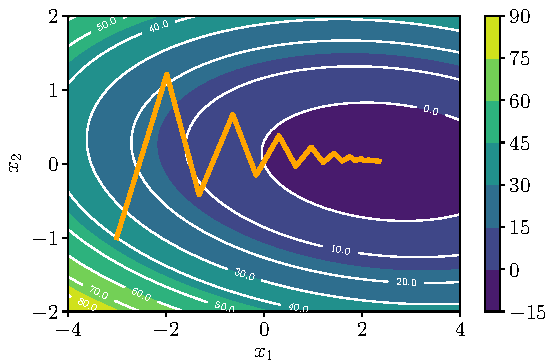
\includegraphics[width=0.5\linewidth]{img/_gradient_contour.pdf}
    \caption{Descent method steps in $\mathbb{R}^2$ (i.e. moving across contour lines)}
\end{figure}


\subsection{Choice of the search direction}

\begin{description}
    \item[Descent direction] \marginnote{Descent direction}
        $\vec{p} \in \mathbb{R}^N$ is a descent direction of $f$ in $\vec{x}$ if:
        \[ \exists \bar{\alpha} > 0, \forall \alpha \in [0, \bar{\alpha}]: f(\vec{x} + \alpha \vec{p}) < f(\vec{x}) \]
\end{description}

\begin{theorem}
    Let $\vec{p} \in \mathbb{R}^N$, $\vec{p} \neq \nullvec$.
    \[ \text{If } \vec{p}^T \nabla f(\vec{x}) < 0 \Rightarrow \vec{p} \text{ descent direction of } f \text{ in } x \]
\end{theorem}

\begin{theorem}
    For all $\vec{x}$, $\vec{p} = -\nabla f(\vec{x})$ is a descent direction of $f$ in $x$.
\end{theorem}
\begin{proof}
    \[
        \begin{split}
            \vec{p}^T \nabla f(\vec{x}) < 0 &\iff -(\nabla f(\vec{x}))^T \nabla f(\vec{x}) < 0 \\
                &\iff - \Vert \nabla f(\vec{x}) \Vert_2^2 < 0
        \end{split}
    \]
    This holds as the norm is always positive.
\end{proof}

\begin{description}
    \item[Gradient-like methods] \marginnote{Gradient-like methods}
        Gradient-like methods are descent methods that use $-\nabla f$ as step.
\end{description}


\subsection{Choice of the step length}
\begin{description}
    \item[Constant] 
        In machine learning, it is common to set a constant value for the step (learning rate), 
        but it can be proved that this does not guarantee convergence.
    
    \item[Backtracking procedure] \marginnote{Backtracking procedure}
        $\alpha_k$ is chosen such that it respects the Wolfe condition\footnote{\url{https://en.wikipedia.org/wiki/Wolfe_conditions}}:
        \begin{lstlisting}[mathescape=true, belowskip = -0.8\baselineskip]
            def backtracking($\tau$, $c_1$):
                $\alpha_k$ = 1 # Initial guess
                while $f(x_k + \alpha_k \nabla f(\vec{x}_k))$ > $f(\vec{x}_k)$ + $c_1 \alpha_k \nabla f(\vec{x}_k)^T \nabla f(\vec{x}_k)$:
                    $\alpha_k$ = $\alpha_k$ / $\tau$
                return $\alpha_k$
        \end{lstlisting}
        It can be proved that, by using the backtracking procedure, gradient methods converge to a local minimum.
\end{description}


\subsection{Stopping condition}
\marginnote{Stopping condition}
We can stop iterating when $\vec{x}_k \approx \vec{x}^*$, that is, when $\nabla f(\vec{x}_k) \approx \nullvec$.
We can verify this by checking the norm of the gradient against a tolerance $\tau$:
\begin{descriptionlist}
    \item[Absolute condition] $\Vert \nabla f(x_k) \Vert_2 < \tau$ 
    \item[Relative condition] $\frac{\Vert \nabla f(x_k) \Vert_2}{\Vert \nabla f(x_0) \Vert_2} < \tau$ 
\end{descriptionlist}

A generic gradient-like method can then be defined as:
\begin{lstlisting}[mathescape=true]
    def gradientMethod($f$, $\vec{x}_0$):
        $k$ = 0
        while stoppingCondition($f$, $\vec{x}_k$, $\vec{x}_0$):
            $p_k$ = $-\nabla f(\vec{x}_k)$
            $\alpha_k$ = backtracking($\dots$)
            $\vec{x}_{k+1}$ = $\vec{x}_k$ + $\alpha_k \vec{p}_k$
            $k$ = $k$ + 1
        return $x_k$
\end{lstlisting}


\subsection{Problems}

\begin{description}
    \item[Choice of the initialization point] \marginnote{Initialization point}
        The starting point of an iterative method is a user-defined parameter.
        For simple problems, it is usually chosen randomly in $[-1, +1]$.
        
        For complex problems, the choice of the initialization point is critical as 
        it may cause numerical instabilities or bad results.
        Heuristics can be used to select an adequate starting point.

    \item[Flat regions and local optima] \marginnote{Flat regions and local optima}
        Flat regions slow down the learning speed,
        while a local optima causes the method to converge at a poor solution.
        \begin{figure}[H]
            \centering
            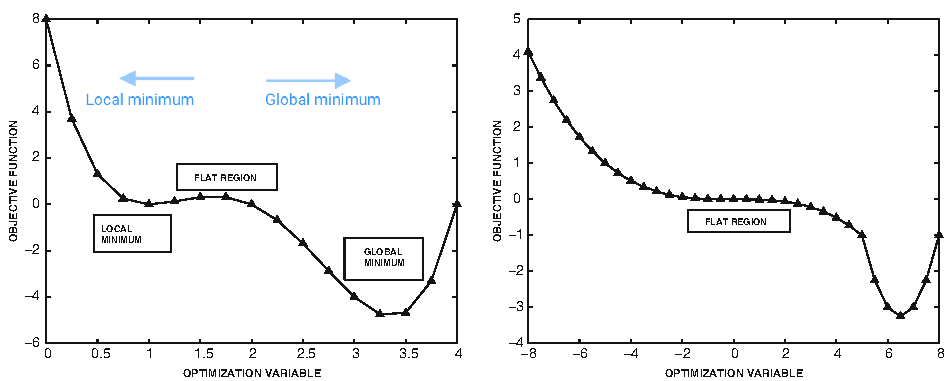
\includegraphics[width=0.9\textwidth]{img/_descent_local_flat.pdf}
            \caption{Flat regions and local minima}
        \end{figure}
    
    \item[Differential curvature]
        Different magnitudes of the partial derivatives may cause the problem of
        vanishing and exploding gradient. \marginnote{Vanishing gradient\\Exploding gradient}
        This causes the learning process to require more iterations to adjust the direction.

        In practice, as the gradient of complex functions is only an instantaneous direction of best decrease and
        does not represent the direction to the minimum in the long term, 
        many updates are required for a gradient method to converge.

        A method to mitigate this issue is to use feature normalization techniques.

    \item[Non-differentiable objective function]
        If the objective function has a small number of non-differentiable points,
        the gradient descent method can be applied with minor modifications.
        
        If lots of points are non-differentiable, the gradients will not be informative enough 
        to determine a decrease direction.

    \item[Difficult topologies]
        \marginnote{Cliff}
        A cliff in the objective function causes problems when evaluating the gradient at the edge.
        With a small step size, there is a slowdown in convergence. 
        With a large step size, there is an overshoot that may cause the algorithm to diverge.
        % a slowdown when evaluating 
        % the gradient at the edge using a small step size and 
        % an overshoot when the step is too large.

        \marginnote{Valley}
        A valley in the objective function causes a gradient method to bounce between the sides
        to a point where no significant progress can be made.

        \begin{figure}[H]
            \begin{subfigure}{.5\textwidth}
                \centering
                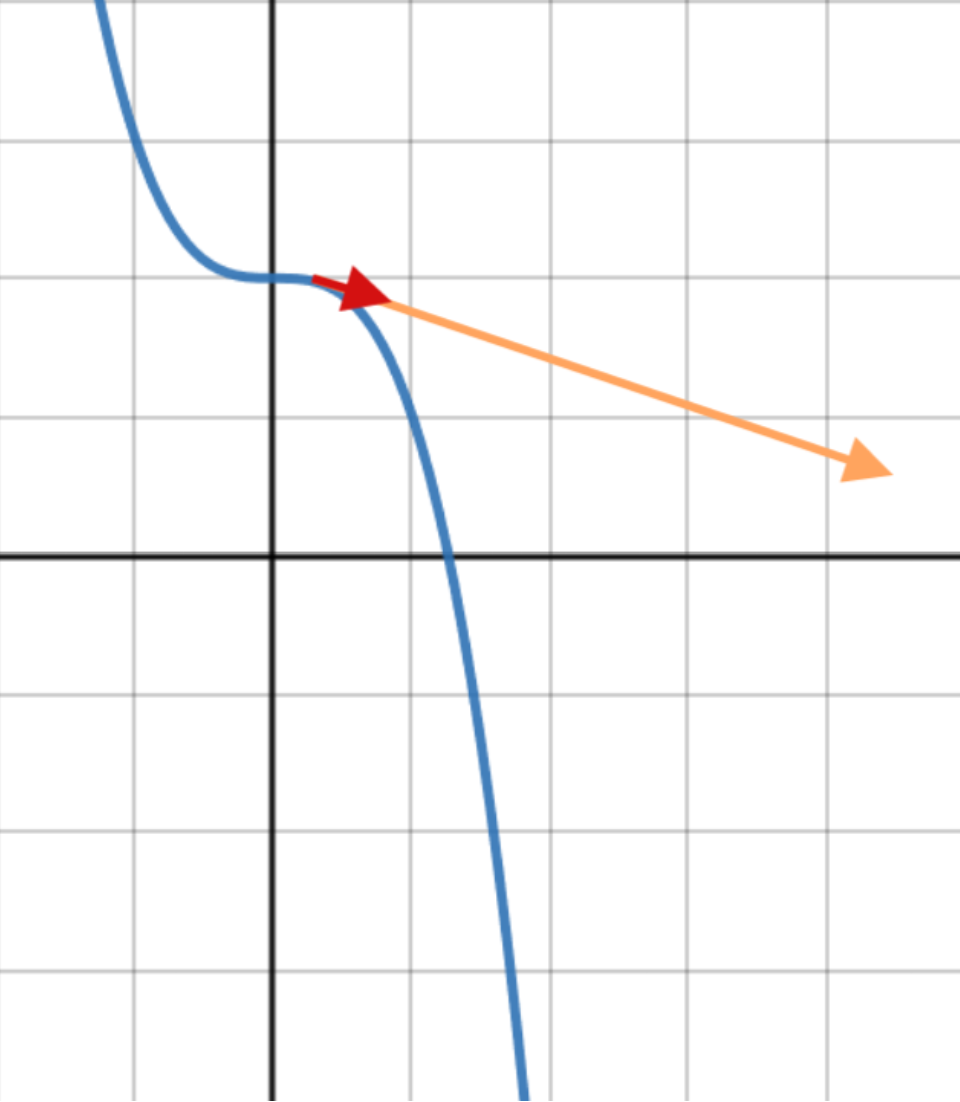
\includegraphics[width=.30\linewidth]{img/cliff.png}
                \caption{Cliff region}
            \end{subfigure}%
            \begin{subfigure}{.5\textwidth}
                \centering
                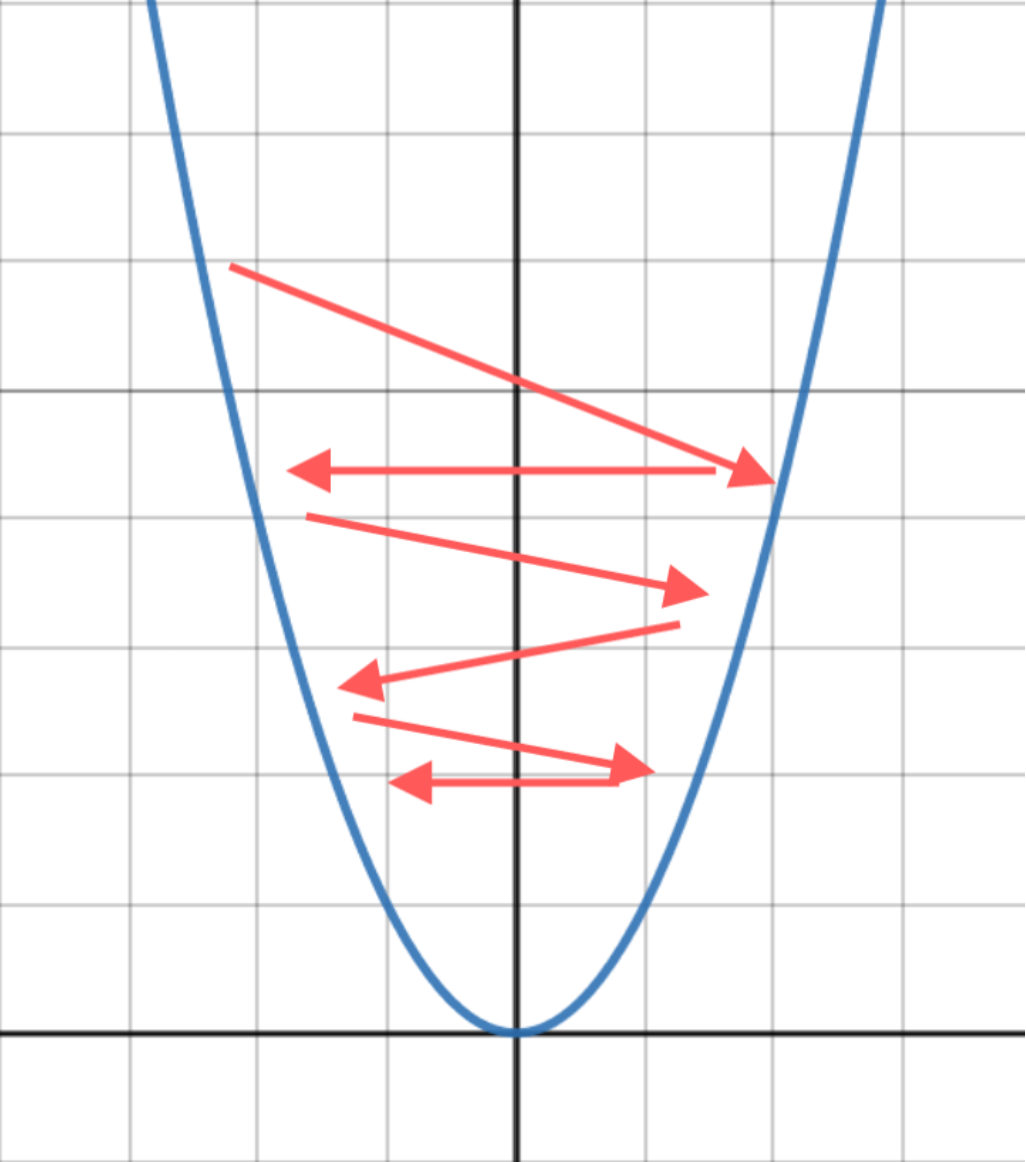
\includegraphics[width=.30\linewidth]{img/valley.png}
                \caption{Ping pong tournament in a valley}
            \end{subfigure}
        \end{figure}
\end{description}



\section{Convex functions}

\begin{description}
    \item[Convex set] \marginnote{Convex set}
        Informally, a set is convex if, for any two points of the set,
        the points laying on the segment connecting them are also part of the set.

        \begin{figure}[H]
            \begin{subfigure}{.5\textwidth}
                \centering
                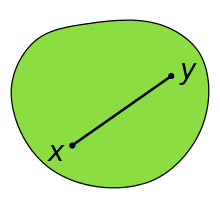
\includegraphics[width=.25\linewidth]{img/convex_set.png}
                \caption{Convex set}
            \end{subfigure}%
            \begin{subfigure}{.5\textwidth}
                \centering
                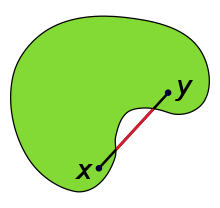
\includegraphics[width=.25\linewidth]{img/non_convex_set.png}
                \caption{Non-convex set}
            \end{subfigure}
        \end{figure}

    \item[Convex function] \marginnote{Convex function}
        Let $\Omega \subseteq \mathbb{R}^n$ be a convex set and $f: \Omega \rightarrow \mathbb{R}$.
        $f$ is convex if:
        \[ 
            \forall \vec{x}_1, \vec{x}_2 \in \Omega, \forall t \in [0, 1]: 
                f(t\vec{x}_1 + (1-t)\vec{x}_2) \leq t f(\vec{x}_1) + (1-t) f(\vec{x}_2)
        \]

        In other words, the segment connecting two points of the function lays above the graph.
        \begin{figure}[H]
            \centering
            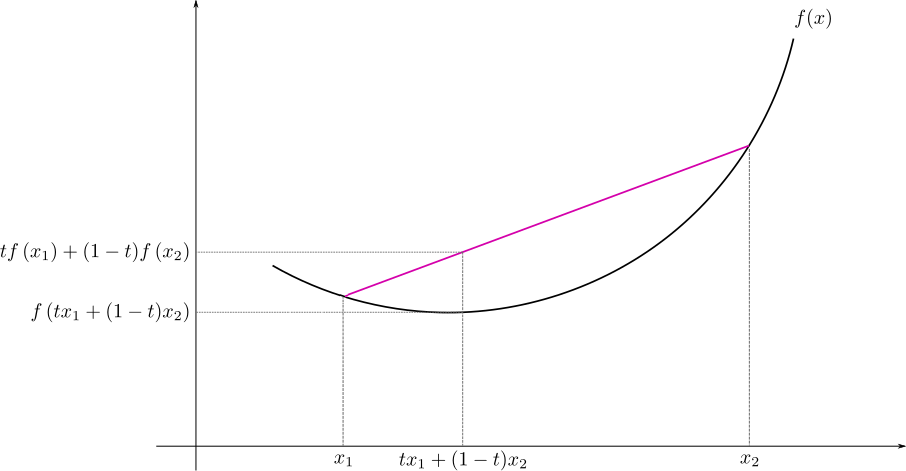
\includegraphics[width=0.55\textwidth]{img/convex_function.png}
            \caption{Convex function}
        \end{figure}

    \item[Strictly convex function] \marginnote{Strictly convex function}
        Let $\Omega \subseteq \mathbb{R}^n$ be a convex set and $f: \Omega \rightarrow \mathbb{R}$.
        $f$ is strictly convex if:
        \[ 
            \forall \vec{x}_1, \vec{x}_2 \in \Omega, \forall t \in [0, 1]: 
                f(t\vec{x}_1 + (1-t)\vec{x}_2) < t f(\vec{x}_1) + (1-t) f(\vec{x}_2)
        \]
\end{description}


\subsection{Properties}
% \marginnote{Convex properties}
\begin{itemize}
    \item $\text{if } f \text{ convex} \Rightarrow \text{any local minimum of } f \text{ is also global}$
    \item $\text{if } f \text{ strictly convex} \Rightarrow \text{the global minimum of } f \text{ is unique}$
    \item $\text{if } f \text{ convex and differentiable} \Rightarrow \text{any stationary point of } f \text{ is a global minimum}$
\end{itemize}


\subsection{Quadratic functions}
\marginnote{Quadratic function}
A quadratic function has form:
\[ f(\vec{x}) = \frac{1}{2}\vec{x}^T\matr{A}\vec{x} - \vec{x}^T\vec{b} + c \]
where $\matr{A} \in \mathbb{R}^{n \times n}$, $\vec{b} \in \mathbb{R}^n$ and $c \in \mathbb{R}$.

\begin{theorem}
    If $f$ is a quadratic form with $\matr{A} \in \mathbb{R}^{n \times n}$ symmetric positive semidefinite,
    then $f$ is convex.
\end{theorem}

\begin{theorem}
    If $f$ is a quadratic form with $\matr{A} \in \mathbb{R}^{n \times n}$ symmetric positive definite,
    then $f$ is strictly convex.
\end{theorem}

\begin{theorem}
    \marginnote{Least squares quadratic function}
    The least squares problem $\Vert \matr{A}\vec{x} - \vec{b} \Vert_2^2$ is a quadratic function.
\end{theorem}
\begin{proof}
    \[
        \begin{split}
            (\matr{A}\vec{x} - \vec{b})^T(\matr{A}\vec{x} - \vec{b}) &= (\vec{x}^T\matr{A}^T - \vec{b}^T)(\matr{A}\vec{x} - \vec{b}) \\
                &= \vec{x}^T\matr{A}^T\matr{A}\vec{x} - \vec{b}^T\matr{A}\vec{x} - \vec{x}^T\matr{A}^T\vec{b} + \vec{b}^T\vec{b} \\
        \end{split}
    \]
    As $\vec{b}^T\matr{A}\vec{x} = \vec{x}^T\matr{A}^T\vec{b}$, we have:
    \[ \vec{x}^T\matr{A}^T\matr{A}\vec{x} - 2\vec{x}^T\matr{A}^T\vec{b} + \vec{b}^T\vec{b} \]

    Let $\matr{B} = \matr{A}^T\matr{A}$, $\vec{q} = \matr{A}^T\vec{b}$ and $c = \vec{b}^T\vec{b}$, 
    we have the quadratic form:
    \[ \vec{x}^T\matr{B}\vec{x} - 2\vec{x}^T\vec{q} + c \]

    $\matr{B}$ is symmetric positive semidefinite (i.e. $\Vert \matr{A}\vec{x} - \vec{b} \Vert_2^2$ is convex).
    Moreover, when $\matr{A}$ is full-rank, $\matr{B}$ is symmetric positive definite (i.e. strictly convex).
\end{proof}



\section{Gradient descent with momentum}
\marginnote{Momentum}
The momentum is an additional term to keep track of previous iterations:
\[
    \Delta \vec{x}_k = \vec{x}_k - \vec{x}_{k-1} = \gamma \Delta \vec{x}_{k-1} - \alpha_{k-1}\nabla f(\vec{x}_{k-1})
\]
where $\gamma \in [0, 1]$. An iteration is therefore defined as:
\[
    \vec{x}_k = \vec{x}_{k-1} - \alpha_{k-1}\nabla f(\vec{x}_{k-1}) + \gamma \Delta\vec{x}_{k-1}
\]



\section{Stochastic gradient descent (SGD)}
\marginnote{Stochastic gradient descent}
SGD is a stochastic approximation of gradient descent that uses an approximation of the gradient.
Given $N$ data points, the loss can be defined as the sum of the individual losses:
\[ L(\vec{x}) = \sum_{n=1}^{N} L_n(\vec{x}) \]
where $\vec{x}$ is the vector of parameters.
The corresponding gradient can be computed as:
\[ \nabla L(\vec{x}) = \sum_{n=1}^{N} \nabla L_n(\vec{x}) \]

\marginnote{Mini-batch}
SGD reduces the amount of computation by approximating the gradient with a subset (mini-batch) $B$ of $\nabla L_n$:
\[ \nabla L(\vec{x}) = \sum_{i \in B} \nabla L_i(\vec{x}) \]

\begin{theorem}
    Under some assumptions and with an appropriate decrease in learning rate, 
    SGD is guaranteed to converge to a local minimum.
\end{theorem}

Different sizes of the mini-batch result in different behavior:
\begin{descriptionlist}
    \item[Large mini-batches] accurate estimates of the gradient.
    \item[Small mini-batches] faster computation.
\end{descriptionlist}